\documentclass[theme=editorial,publication-type=feature-article]{reportkit}
% ReportKit example: feature-article publication type + editorial theme.
% Phase E of docs/superpowers/specs/2026-09-09-reportkit-multi-format-publication-architecture-spec.md
% (sections 12.3, 15 and 18). Everything in this article is fictional:
% Varenholm, its delta, its people, the Tideline Quarterly and every number
% are invented for the fixture and reproduce no third-party branding.
%
% The source below uses only the feature-article semantic primitives
% (featureopening, featureheadline, featuredeck, featurebyline,
% openingvisual, dropcap, featuresection, featurecolumns, pullquote,
% featuresidebar, featureexhibit, imagecredit, featurereferences) and the
% shared diagram/chart layer. There are no coordinates, local font or color
% changes, or raw minipage layouts. tests/test_editorial_theme.py compiles
% this exact file a second time with only the theme= option swapped for an
% unrelated probe theme -- the Phase E gate.
%
% Regenerate figures/ with:
%   PYTHONPATH=python_scripts python3 latex_templates/examples/editorial-feature/figures.py
\setreportkitleftheader{Tideline Quarterly}
\setreportkitfooter{Tideline Quarterly \textperiodcentered\ Autumn issue}
\setreportkitversion{Fictional example}
\setreportkitsubject{Feature article: flood measurement in a fictional delta town}
\setreportkitkeywords{ReportKit, feature article, editorial, fictional example}
\setreportkitlanguage{en-US}
\title{The river that learned to count}
\author{Mara Ellison}
\date{}

\begin{document}

\begin{featureopening}
\featureheadline[Infrastructure]{The river that learned to count}
\featuredeck{For a century the delta town of Varenholm fought its floods with sandbags and memory. Then a harbour engineer, a retired schoolteacher and forty cheap gauges changed what the town argued about.}
\featurebyline{By Mara Ellison}[Field report \textperiodcentered\ 14-minute read]
\begin{openingvisual}{A survey drawing of the Varen delta: five braided channels running from the upland to the sea, with the forty gauge stations installed between 2019 and 2026 marked along them.}[Illustration: Tideline Quarterly, from the Varenholm gauge survey]
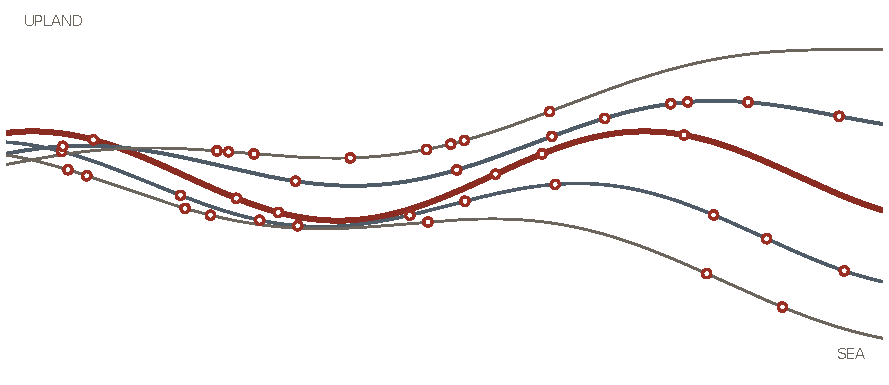
\includegraphics[width=\linewidth]{figures/opening-delta.pdf}
\end{openingvisual}
\end{featureopening}

\dropcap{T}{he river} rose twice that spring before anyone thought to measure it. The first time, in late March, it came up quietly overnight and left a brown line on the bakery wall on Quay Street, a hand's width below the line from the year before. The second time it came up in the afternoon, fast and loud, and by the time the church bell rang the warning the water was already over the lower steps of the harbour office. Nobody drowned. Three houses on the Salt Flats were ruined, the ferry landing was shut for a month, and the town council held the same meeting it had held, in one form or another, for most of a century.

That meeting always had the same shape. Someone from the upland farms said the dredging had been neglected. Someone from the harbour said the farms had drained too much of the marsh. The fire chief said, correctly, that nobody could prove either claim, and that the only thing that had ever reliably worked was a person standing on the old stone bridge watching the water and ringing the bell. The council voted money for sandbags. The minutes, which go back to 1911, record the vote in nearly identical words forty-three times.

This is the story of how that meeting stopped happening. It is not a story about a dramatic piece of engineering. The thing that changed Varenholm cost less than a single season of sandbags, and most of it was bolted to fence posts.

\featuresection{Counting the water}[The first gauge was a plastic pipe, a pressure sensor and a solar panel the size of a paperback. It cost less than a single sandbag wall.]

\begin{featurecolumns}
Ilse Marten spent thirty-one years teaching mathematics at the Varenholm secondary school and, by her own account, never once thought about the river. “It was just there,” she told me, standing on the bridge in a borrowed raincoat. “You knew which streets flooded the way you knew which teachers were strict. It was local knowledge. Nobody wrote it down.”

What changed her mind was a student project. In the autumn after the spring floods, a group of her final-year students built a water-level gauge for a science fair: a length of plastic pipe sunk into the riverbank, a cheap pressure sensor at the bottom, and a small radio that sent a reading every ten minutes to a laptop in the classroom. It won nothing. But the laptop stayed on, and over the winter it drew a line that nobody in the town had ever seen: the river breathing.

“It went up and down with the tide, of course,” Marten said. “Everybody knew that. What nobody knew was that before every bad day there was a small bump, eight or nine hours earlier, when the upland streams started to fill. It was right there. It was just too small to see from the bridge.”

She took the graph to the harbour office, where it landed on the desk of Tomas Reyk, the harbour engineer, who had been asking the council for a monitoring system for eleven years. The quotes he had collected started at a figure larger than the town's entire annual maintenance budget. The student gauge, including the pipe, had cost about the same as a good pair of boots.

\pullquote{We stopped arguing about the river once we could see it.}[Tomas Reyk, harbour engineer]

Reyk did not trust it. “My first reaction was that a school project cannot be infrastructure,” he said. “Infrastructure has to work at three in the morning in a storm when nobody is looking at it.” So he did what engineers do with things they do not trust: he tried to break it. He sank a second gauge beside the first, then a third on the far bank, and compared their readings for a month. They agreed with each other, and with his tide tables, to within a centimetre.

By the following summer there were twelve gauges along the main channel. By the end of the second year there were forty, spread across all five braids of the delta, most of them bolted to fence posts and farm gates whose owners had agreed, sometimes after considerable persuasion, to host them.

\begin{featuresidebar}{How the gauges work}
Each station is a sealed pipe sunk into the bank with a pressure sensor at its foot. The sensor reports the height of the water above it every ten minutes over a low-power radio link.

A small solar panel keeps the battery charged; in winter a station can run for about three weeks without sun.

Readings are relayed through two repeaters on the church tower and the grain silo to a server in the harbour office, which publishes them on a public page. The whole design, parts list and code are published by the school so that any station can be rebuilt by hand.
\end{featuresidebar}

The distribution of those forty stations was itself a small political achievement. Old Harbour, the district that floods first and worst, has the most. The upland farms, whose owners had spent decades being blamed for the floods, ended up hosting the stations that most often raised the first alarm.

\begin{featureexhibit}{Old Harbour carries the densest part of the network}
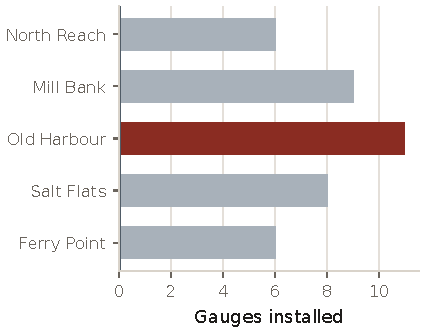
\includegraphics[width=\linewidth]{figures/gauges-by-district.pdf}
\imagecredit{Source: Varenholm gauge survey, fictional data}
\end{featureexhibit}
\end{featurecolumns}

\featuresection{What the numbers changed}[The gauges did not stop the river. They changed how early the town knew what the river was about to do.]

Before the gauges, the town's warning system was a person on the bridge. It worked, in the sense that people usually got out of the way in time, but the median warning it gave --- the time between the bell and the water reaching the first doorstep --- was a little over three hours. That is enough time to move a car, and not enough to move a shop.

With the network in place, the warning starts upstream. When the upland stations register the first rise, the harbour server compares it with the pattern of past floods and, if the shape matches, sends a message to the fire chief and to a list of volunteers. By the sixth year of the network the median lead time had risen to more than fourteen hours.

The difference is not abstract to the people who live with it. Fourteen hours is long enough to lift stock onto upper shelves, move the ferry to the upland mooring and empty the ground floor of the care home on Mill Bank, which in the old days was evacuated in the dark by torchlight. The owner of the bakery on Quay Street, whose wall still carries the brown lines of earlier floods, now closes early on warning days and has not lost a batch of flour since the network reached the upland streams.

Lead time also changed who gets warned. Under the bell, the warning reached whoever could hear it: the harbour, the church and the streets around the bridge. Farms on the upland streams, which often flooded first, heard nothing at all. The gauge messages go to a list, and the list is organised by where the water arrives rather than by who lives closest to the bell.

None of this happened because the gauges are clever. Each one measures a single number. What the network added was a record: every rise, every false alarm and every flood, written down in the same way, in the same place, every ten minutes for six years. The harbour office now has more measurements of the Varen than the town collected in the previous century.

\begin{featureexhibit}[span=full]{Forty gauges moved the median flood warning from three hours to more than fourteen}
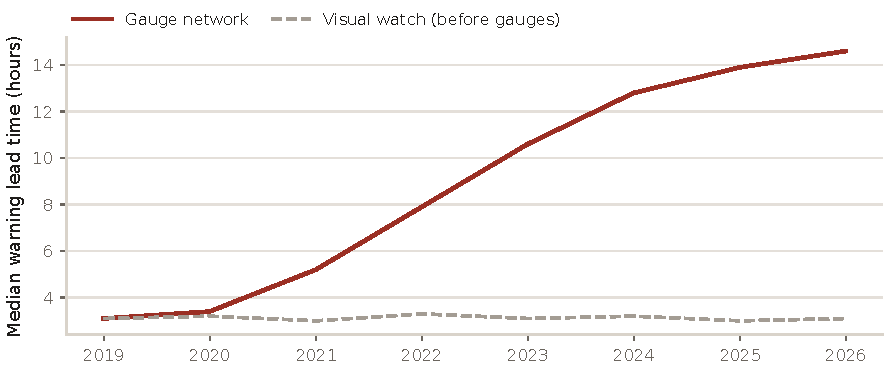
\includegraphics[width=\linewidth]{figures/warning-lead-time.pdf}
\imagecredit{Source: Varenholm harbour office warning log, 2019--2026, fictional data. The visual-watch series is the pre-network baseline observed from the bridge.}
\end{featureexhibit}

The exhibit hides something the harbour office is careful to point out: the gain did not arrive all at once. The first twelve gauges, all on the main channel, added almost nothing. The warning time only began to climb once stations reached the smaller upland streams, which is where the floods actually begin. “The first year proved the gauges worked,” Reyk said. “The second year proved we had put them in the wrong place.”

The path a warning now travels is short, and deliberately boring. Each step has a named owner, and each step can be done by hand if the server fails.

\begin{featureexhibit}{A warning now travels from an upland stream to a doorstep in four steps}
\begin{diagram}[caption={},source={},description={An upland rise is detected by a gauge, matched against past floods by the harbour server, confirmed by the duty officer, and sent to volunteers who knock on doors.}]
\begin{reportflow}
\step{rise}{Upland gauge rises}
\step{match}{Server matches the pattern}
\step{confirm}{Duty officer confirms}
\step{knock}{Volunteers knock}
\flowedge{rise}{match}
\flowedge{match}{confirm}
\flowedge{confirm}{knock}
\end{reportflow}
\end{diagram}
\imagecredit{Diagram: Tideline Quarterly}
\end{featureexhibit}

The last step is the one people in Varenholm talk about. A message on a phone is easy to ignore at three in the morning; a neighbour at the door is not. The volunteer list now runs to about ninety names, organised by street, and the fire chief rings them in the order the water is expected to arrive.

\featuresection{The argument that stopped}[The most surprising result had nothing to do with water. It was what happened to the council meeting.]

\begin{featurecolumns}
The minutes tell the story better than anyone I interviewed. In the three years before the first gauge, the council discussed flooding at fourteen meetings. Almost all of that time was spent on the same question --- whose fault is it? --- and none of it produced anything but sandbags.

In the three years after the network reached the upland streams, flooding came up at nine meetings, and the questions were different. Should the volunteer list be split into two shifts? Could the gauge data be used to time the dredging? Was the Ferry Point station reading high because of silt, or because the bank was moving?

“Once there was a line on a screen, nobody could claim the river did something it did not do,” said Anya Holt, who chaired the council for six of those years. “The farmers could see the upland streams rise first. The harbour could see its own tide. People did not agree about everything. But they agreed about what had happened.”

\pullquote{People did not agree about everything. But they agreed about what had happened.}[Anya Holt, former council chair]

There were costs. Two stations were stolen in the first year, and one was destroyed by a tractor whose driver insisted, with some justification, that it had not been there the day before. The radio repeaters on the church tower needed a permission that took nine months and a visit from the diocese to obtain. And the public page, which anyone can read, has occasionally caused panic when a single faulty sensor spiked.

The harbour office's answer to the last problem is characteristic of the whole project: it publishes the faults too. Every station has a small history of its own failures, visible beside its readings. “If people are going to trust the numbers,” Reyk said, “they have to be able to see when the numbers are wrong.”
\end{featurecolumns}

\featuresection{What travels}[Other delta towns have asked for the design. The harbour office is careful about what it claims.]

Varenholm now receives two or three letters a month from towns along other rivers asking how to copy what it did. The school sends them the parts list. The harbour office sends a longer letter, which says, in effect, that the gauges were the easy part.

The hard part, Reyk argues, was everything the gauges forced into the open: which streams actually flood first, who is responsible for each step of a warning, and what the town does when a station lies. None of that can be bought, and none of it is in the parts list. A town that installs forty gauges and changes nothing else will, he suspects, simply have a very detailed record of its floods.

Marten, who still checks the classroom laptop most mornings, puts it more simply. “The river was always telling us what it was going to do,” she said. “We just had not been listening in the right place.”

On my last evening in Varenholm the river was low and quiet, and the only sound on the old stone bridge was the tick of the bell rope against its post. Nobody has rung that bell for a flood in four years. The town keeps it, and tests it every spring, in case the gauges are ever wrong.

\begin{featurereferences}[Notes and sources]
\item Varenholm Town Council (1911--2026), minutes of council meetings, flooding items. Fictional archive. \url{https://example.com/varenholm/minutes}
\item Varenholm Harbour Office (2026), flood warning log and station fault history, 2019--2026. Fictional dataset. \url{https://example.com/varenholm/warnings}
\item Varenholm Secondary School (2020), open gauge design, parts list and firmware. Fictional publication. \url{https://example.com/varenholm/gauge}
\item Interviews with Ilse Marten, Tomas Reyk and Anya Holt, conducted for this article. All people named are fictional.
\item Lead-time figures are medians of the warning log; the pre-network baseline is the bell-to-doorstep interval recorded by the fire service.
\end{featurereferences}

\end{document}
